\section{Building the Translation Matrices} \label{sec:translation-matrices}

With the foundational mathematics now defined, we can now construct the translation matrices that are the core of the \ac{FMM} algorithm. These operators map the coefficients of an acoustic series expansion centered at one spatial location to an equivalent, physically identical series expansion centered at a new geometric origin.
Using the broadband formulations described by \cite{gumerovbroadbandfastmultipole2009}, the \ac{FMM} framework leverages addition theorems to generate  structured dense matrices for all the necessary translations, including \ac{M2M}, \ac{M2L}, and \ac{L2L} translations. These matrices are precomputed and stored for efficient reuse during the algorithm's execution, significantly reducing the immense computational overhead associated with on-the-fly calculations.
\begin{figure} [htpb] 
    \centering
    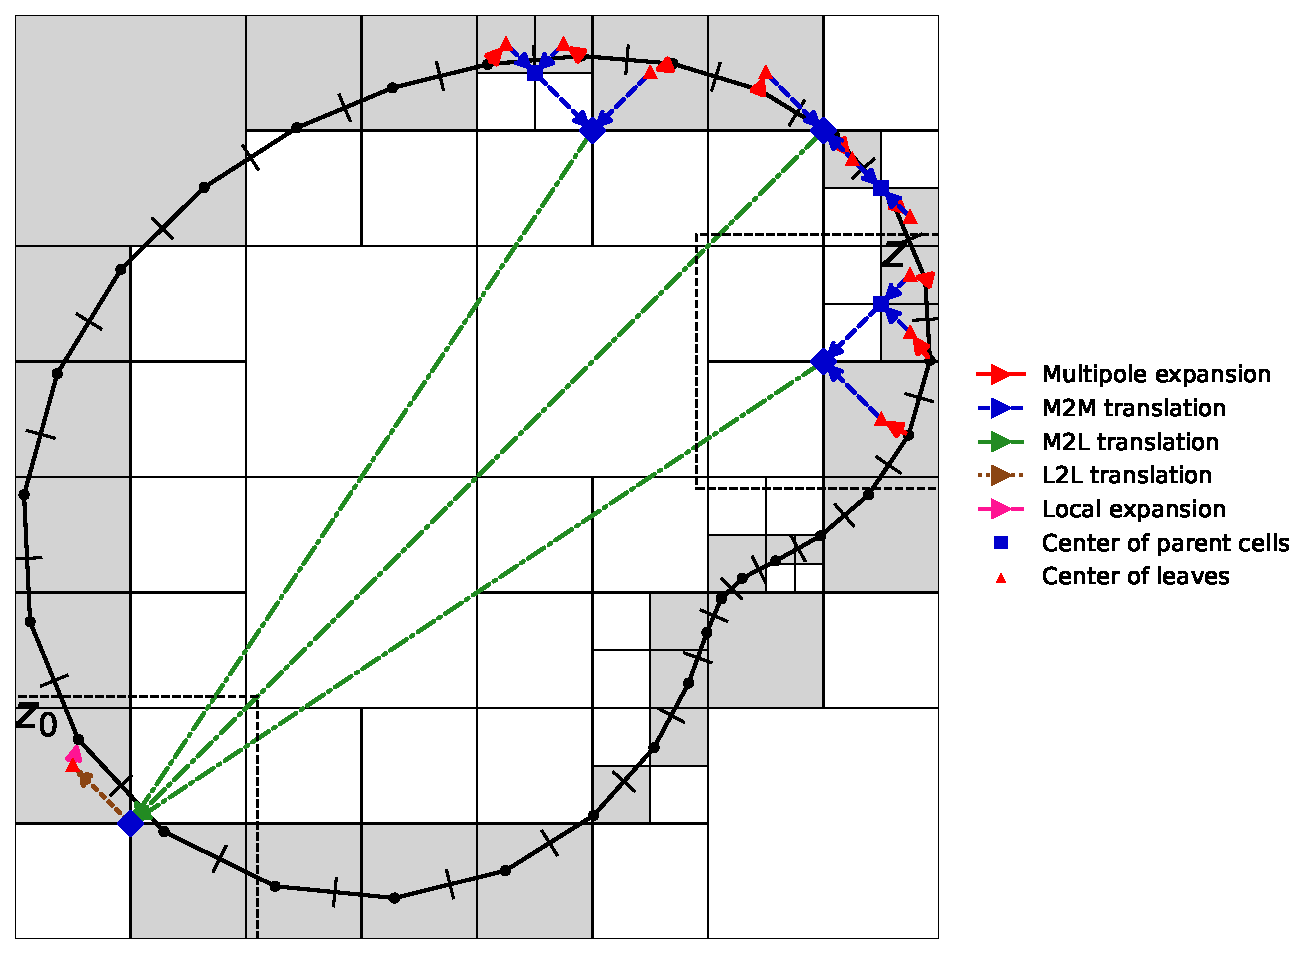
\includegraphics[width=0.8\textwidth]{figures/diagram_3_fmm_main.pdf} 
    \caption{A simplified representation of the FMM algorithm's main steps. This follows the same 2D system from \ref{fig:quadtree-domain} and \ref{fig:quadtree-logical}. We show some of the far-field interactions and how they are computed. The green arrows represent the \ac{M2L} translations, the blue arrows represent the \ac{M2M} translations, and the red arrows represent the Multipole Expansions. The brown arrows represent the \ac{L2L} translations, and the orange arrows represent the \ac{L2P} local expansions. \cite{liufastmultipoleboundary2006}}
    \label{fig:fmm-interaction}
\end{figure}

\begin{figure}[htpb]
    \centering
    \begin{subfigure}[t]{0.48\textwidth}
        \centering
        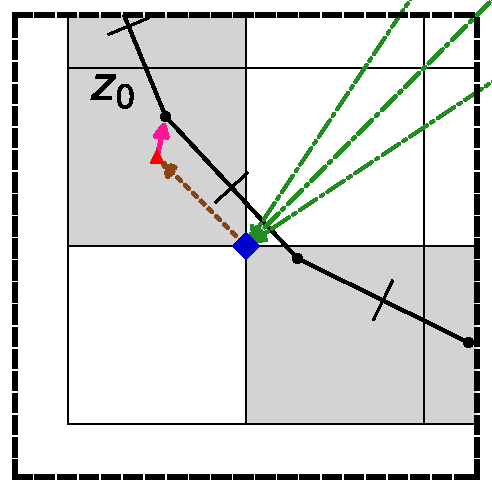
\includegraphics[width=\linewidth]{figures/diagram_4_fmm_target_zoom.pdf} 
        \caption{We can see how the incoming information from the \ac{M2L} interactions is translated down to the leaf node, and the \ac{L2P} local expansion translates it onto the boundary element.}
        \label{fig:fmm-target-zoom}
    \end{subfigure}\hfill
    \begin{subfigure}[t]{0.48\textwidth}
        \centering
        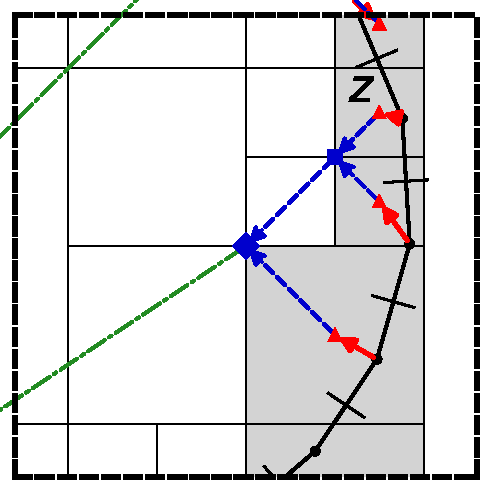
\includegraphics[width=\linewidth]{figures/diagram_5_fmm_source_zoom.pdf} 
        \caption{The upwards translation process, where the multipole expansion of the boundary element is translated up to the leaf node's center, and then up to the parent node's center with the \ac{M2M} translation, before being translated to the far-field node's center with the \ac{M2L} translation.}         
        \label{fig:fmm-source-zoom}
    \end{subfigure}
    \caption{Close up views of the translation process for the target and source nodes from \ref{fig:fmm-interaction} \cite{liufastmultipoleboundary2006}}
    \label{fig:translation-matrices-combined}
\end{figure}

\subsection{Point-to-Multipole (P2M) Translations}
The \ac{P2M} translation is the first step in the upward pass of the \ac{FMM} algorithm. It calculates the influence of the boundary elements within a leaf node and projects them into multipole coefficients relative to the geometric center of the leaf node. 

\newglossaryentry{Multipole Expansion Coefficient}{
    name={$M_{n}^m$},
    description={Specific multipole expansion coefficient for degree $n$ and order $m$}
}
The Collocation method for the \ac{BEM} that we use assigns both potential and flux distributions to boundary elements. This causes the mesh surfaces to act as continuous distributions of acoustic dipole. The multipole coefficients $M_{n}^m$  for an expansion order $P$ are accumulated in a flattened one-dimensional array of size $(P+1)^2$, where the memory index is calculated optimally as $n^2 + n + m$, running linearly from $n=0...P$ and $m=-n...n$.

We implement two methods to compute the source projection, the first is an Analytical method which provides mathematically exact derivatives, and a \ac{FDM} as fallback for numerical stability near singularities.

\subsubsection{The Analytical \ac{P2M}} \label{analytical-p2m}

\newglossaryentry{fnm}{
    name={$f_n^m(r, \theta, \phi)$},
    description={Outgoing multipole basis function for degree $n$ and order $m$}
}
The exact mathematical basis function that represents the outgoing acoustic expansion is given by the product of the regular spherical Bessel function and the complex conjugate of the spherical harmonic function like so:
\begin{equation}
    f_n^m(r, \theta, \phi) = j_n(kr) \overline{Y_n^m(\theta, \phi)}
\end{equation}
The surface dipole source representing the \ac{BEM} double layer formulation requires an operator that is the directional derivative of this basis with respect to the continuous surface element's Cartesian normal vector $n = (n_x, n_y, n_z)$.

To align with the spherical basis, the Cartesian normal is projected into the local spherical components $(n_r, n_\theta, n_\phi)$ through the following standard coordinate transformation:
\begin{align}
    n_r &= n_x \sin\theta \cos\phi + n_y \sin\theta \sin\phi + n_z \cos\theta \\
    n_\theta &= n_x \cos\theta \cos\phi + n_y \cos\theta \sin\phi - n_z \sin\theta \\
    n_\phi &= -n_x \sin\phi + n_y \cos\phi
\end{align}
The required dipole basis can be constructed as the vector dot product of the spherical spatial gradient and the projected normal vector:
\begin{equation}
    \text{dipole\_basis} = \frac{\partial f_n^m}{\partial r} n_r + \frac{1}{r} \frac{\partial f_n^m}{\partial \theta} n_\theta + \frac{1}{r \sin\theta} \frac{\partial f_n^m}{\partial \phi} n_\phi
\end{equation}
The radial gradient component is derived using the derivative recurrence relation for spherical Bessel functions:
\begin{align}
    j'_0(kr) &= -k \cdot j_1(kr) \\
    j'_n(kr) &= k\left( \frac{n \cdot j_n(kr)}{kr} - j_{n+1}(kr) \right) \text{ for }  n > 0
\end{align}
To get the angular gradient components, we need to evaluate the derivatives of the spherical harmonics. The polar derivative $\frac{\partial Y_n^m}{\partial \theta}$  is computed using specialized quantum mechanics ladder operators that link adjacent degree coefficients. The inclusion of the Condon-Shortley phase factor, $(-1)^m$, in the definition of the spherical harmonics is what allows these raising and lowering operators to be applied, vastly improves speed over direct transcendental derivation. The azimuthal derivative $\frac{\partial Y_n^m}{\partial \phi}$ trivially evaluates to $i m Y_n^m$. \cite{eptonmultipoletranslationtheory1995}\cite{messiah1961quantum}

\subsubsection{The \ac{FDM} Fallback} \label{subsubsec:fdm-fallback}

The analytical \ac{P2M} method described in \ref{analytical-p2m} while mathematically exact, can encounter numerical instability when the source point is very close to the expansion center or on its vertical polar axis, as it contains divisions by $r$ and $r\sin\theta$. We have implemented safeguards to detect these edge cases and switch to a finite difference approximation of the normal derivative in these scenarios. The \ac{FDM} implementation uses two infinitesimally offset target points, $p_+ = \text{center} + \epsilon n$ and $p_- = \text{center} - \epsilon n$, and the analytical basis is evaluated at both these points to compute the derivative numerically via the central difference $(f_+ - f_-) / (2\epsilon)$.

\subsection{Gaunt Addition Theorem for Acoustic Waves} \label{subsec:gaunt-addition-theorem}
The \ac{M2M} operators consolidates coefficients from smaller child nodes into large parent nodes, while the \ac{M2L} operators convert the outgoing multipole signatures into incoming localized incident fields across the separated nodes of the interaction lists. 
The \ac{M2L} and the \ac{M2M} translations are fundamentally reliant on the exact formulations based on Gaunt addition theorems.
The theorem defines the mechanism by which a target multipole coefficient is generated by multiplying the entire spectrum of source coefficients by a specific transformation matrix based on their spatial separation vector $d$.

Let the displacement vector between the translation centers be defined in local spherical coordinates as $(r, \theta, \phi)$. Following the analytical derivations laid out by Gumerov and Duraiswami \cite{gumerovbroadbandfastmultipole2009}, the specific scalar entry for the transformation matrix ($T_{entry}$), which links the $(n', m')$ source mode to the $(n, m)$ target mode, requires an internal summation over a third intermediate index $p$. The bounds of $p$ are strictly dictated by the Wigner triangle inequality $|n-n'| \leq p \leq n+n'$ \cite{gumerovrecursionscomputationmultipole2004}.

\newglossaryentry{Tentry}{
    name={$T_{entry}$},
    description={Specific scalar entry in a translation matrix linking source and target multipole coefficients}
}

The matrix entry $T_{entry}$ is accumulated as:
\begin{equation}
    T_{entry} = \sum_{p} 4\pi i^{n' - n + p} \cdot (-1)^{m'} \cdot G(n, m; n', -m'; p) \cdot z_p(kr) \cdot Y_p^{m-m'}(\theta, \phi)
\end{equation}

\newglossaryentry{Zp}{
    name={$z_p(kr)$},
    description={Generalized target spherical radial function for degree $p$ and wavenumber $k$ used in the addition theorems (can be a Bessel or Hankel function depending on the operator type)}
}
Each component in this equation has a specific mathematical and physical significance:
\begin{itemize}
    \item Integration prefactor $4\pi$ scales the translation to the appropriate solid angle.
    \item The complex exponential term $i^{n' - n + p}$  dictates the interference pattern of the translated wave. To avoid having to compute expensive complex exponentials, we leverage the fact that $i^k$ cycles through the values $\{1, i, -1, -i\}$ every four increments of $k$, allowing us to compute this term with a simple modulo operation and a small lookup table.
    \item The parity selection rules embedded within the Gaunt coefficient $G$ automatically skip all iterations where $(n + n' + p)$ is an odd integer. This effectively halves the number of required summation loops.
    \item The term $z_p(kr)$ represents the appropriate spherical radial function, dependent entirely on the operator type.
\end{itemize}

\subsection{Formulating the \ac{M2M}, \ac{M2L}, and \ac{L2L} Translation Operators} \label{subsec:operator-formulation}
By simply varying the choice of the spherical radial function $z_p(kr)$, the generic addition theorem described above in \ref{subsec:gaunt-addition-theorem} can be used to construct the specific operators required for the \ac{FMM} passes as shown in \autoref{tab:translation_operators}.
\begin{table}[htbp]
\centering
\small % Slightly reduces font size to fit text better
\renewcommand{\arraystretch}{1.4} % Adds a bit of padding to the rows
\setlength{\tabcolsep}{8pt} 
% The sum of \hsize fractions (0.7 + 0.8 + 1.5) must equal the number of X columns (3)
\begin{tabularx}{\textwidth}{ 
    >{\hsize=0.7\hsize}L 
    >{\hsize=0.8\hsize}L
    >{\hsize=0.8\hsize}L 
    >{\hsize=1.7\hsize}L 
}
\toprule
\textbf{Operator Type} & \textbf{Application} & \textbf{Target Function $z_p(kr)$} & \textbf{Computational Characteristics} \\
\midrule
M2M Matrix & Upward Pass \newline (Child to Parent)   & Regular Bessel $j_p(kr)$        & Translates within a continuous, finite domain. Exact shift of geometric center. \\
M2L Matrix & Horizontal Pass \newline (Across lists)  & Singular Hankel $h_p^{(1)}(kr)$ & Translates across the void between well-separated nodes, modeling the required outward acoustic radiation. \\
L2L Matrix & Downward Pass \newline (Parent to Child) & Regular Bessel $j_p(kr)$        & Translates the incident local field deeper into the spatial subdivision. \\
\bottomrule
\end{tabularx}
\caption{Translation Operators and Computational Characteristics}
\label{tab:translation_operators}
\end{table}

Since we enforce a fixed uniform expansion order $P$ across the entire tree, the dimensionality of all these translation matrices is locked to $(P+1)^2 \times (P+1)^2$. All these matrices are precomputed once, cached in memory, and applied sequentially to the dynamically changing coefficient vectors during each \acs{GMRES} iteration.